\documentclass[crop,tikz]{standalone}
\usetikzlibrary{positioning,arrows,fit,calc}
\pgfdeclarelayer{bg}
\pgfsetlayers{bg,main}
\tikzset{
	>=stealth'
}
\begin{document}
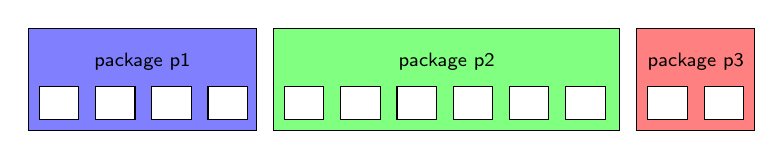
\begin{tikzpicture}[
node distance = 2mm,
every node/.style = {
	font = \sffamily\scriptsize
},
jar/.style = {
	draw,
	minimum height = 2.cm
},
package/.style = {
	draw,
	minimum height = 1.3cm,
	minimum width = 1.5cm
},
class/.style = {
	draw,
	fill = white,
	minimum height = \baselineskip,
	minimum width = .5cm
}
]

\node (package_1) [package, fill=blue!50, minimum width = 29mm] {};
\node [below = of package_1.north] {package p1};
\node (class_1) [class, above right = of package_1.south west] {};
\node (class_2) [class, right = of class_1] {};
\node (class_3) [class, right = of class_2] {};
\node (class_4) [class, right = of class_3] {};

\node (package_2) [package, right = of package_1, fill=green!50, minimum width = 44mm] {};
\node [below = of package_2.north] {package p2};
\node (class_5) [class, above right = of package_2.south west] {};
\node (class_6) [class, right = of class_5] {};
\node (class_7) [class, right = of class_6] {};
\node (class_8) [class, right = of class_7] {};
\node (class_9) [class, right = of class_8] {};
\node (class_10) [class, right = of class_9] {};


\node (package_3) [package, right = of package_2, fill=red!50] {};
\node [below = of package_3.north] {package p3};
\node (class_11) [class, above right = of package_3.south west] {};
\node (class_12) [class, right = of class_11] {};

\end{tikzpicture}

\end{document}